\begin{exercises}
	
\exercise 设$\varPsi_{1}(\boldsymbol{r},t)$和$\varPsi_{2}(\boldsymbol{r},t)$是两个真实的运动态波函数,满足薛定谔方程.证明$\int_{\text{全}}\varPsi_{1}^{*}\varPsi_{2}d\tau$之值与时间无关.
	
\exercise 证明从单粒子薛定谔方程解出的速度场是无旋的,即$\nabla\times \boldsymbol{v}=0$,其中$\boldsymbol{v}=\dfrac{\boldsymbol{j}}{\rho}$,$\rho$为概率密度,$\boldsymbol{j}$为概率流密度.
	
\exercise 粒子在一维势场$V(x)$中运动,$V(x)$无奇点.设$\varPsi_{n}(x)$,$\varPsi_{m}(x)$为束缚态波函数,$E_{n}\neq E_{m}$.证明$\varPsi_{n}$与$\varPsi_{m}$正交,即证明
\begin{empheq}{equation*}
	\int_{-\infty}^{\infty}\varPsi_{n}(x)\varPsi_{m}(x)dx=0
\end{empheq}
	
\exercise 同上题,证明方程$\varPsi_{n}(x)=0$的根都是单根.
	
$\big[$提示:利用泰勒展开,并对薛定谔方程求导,证明:如$\varPsi_{n}(x)$有2级以上零点,则$\varPsi_{n}(x)$恒等于0.$\big]$
	
\exercise\label{ex2.5} 质量为$m$的粒子被限制在$0<x<a$(无限深势阱)运动,求全部束缚态能级($E_{n}$)和归一化波函数($\varPsi_{n}$).
	
\begin{wrapfigure}[6]{r}{10em}
	\centering
	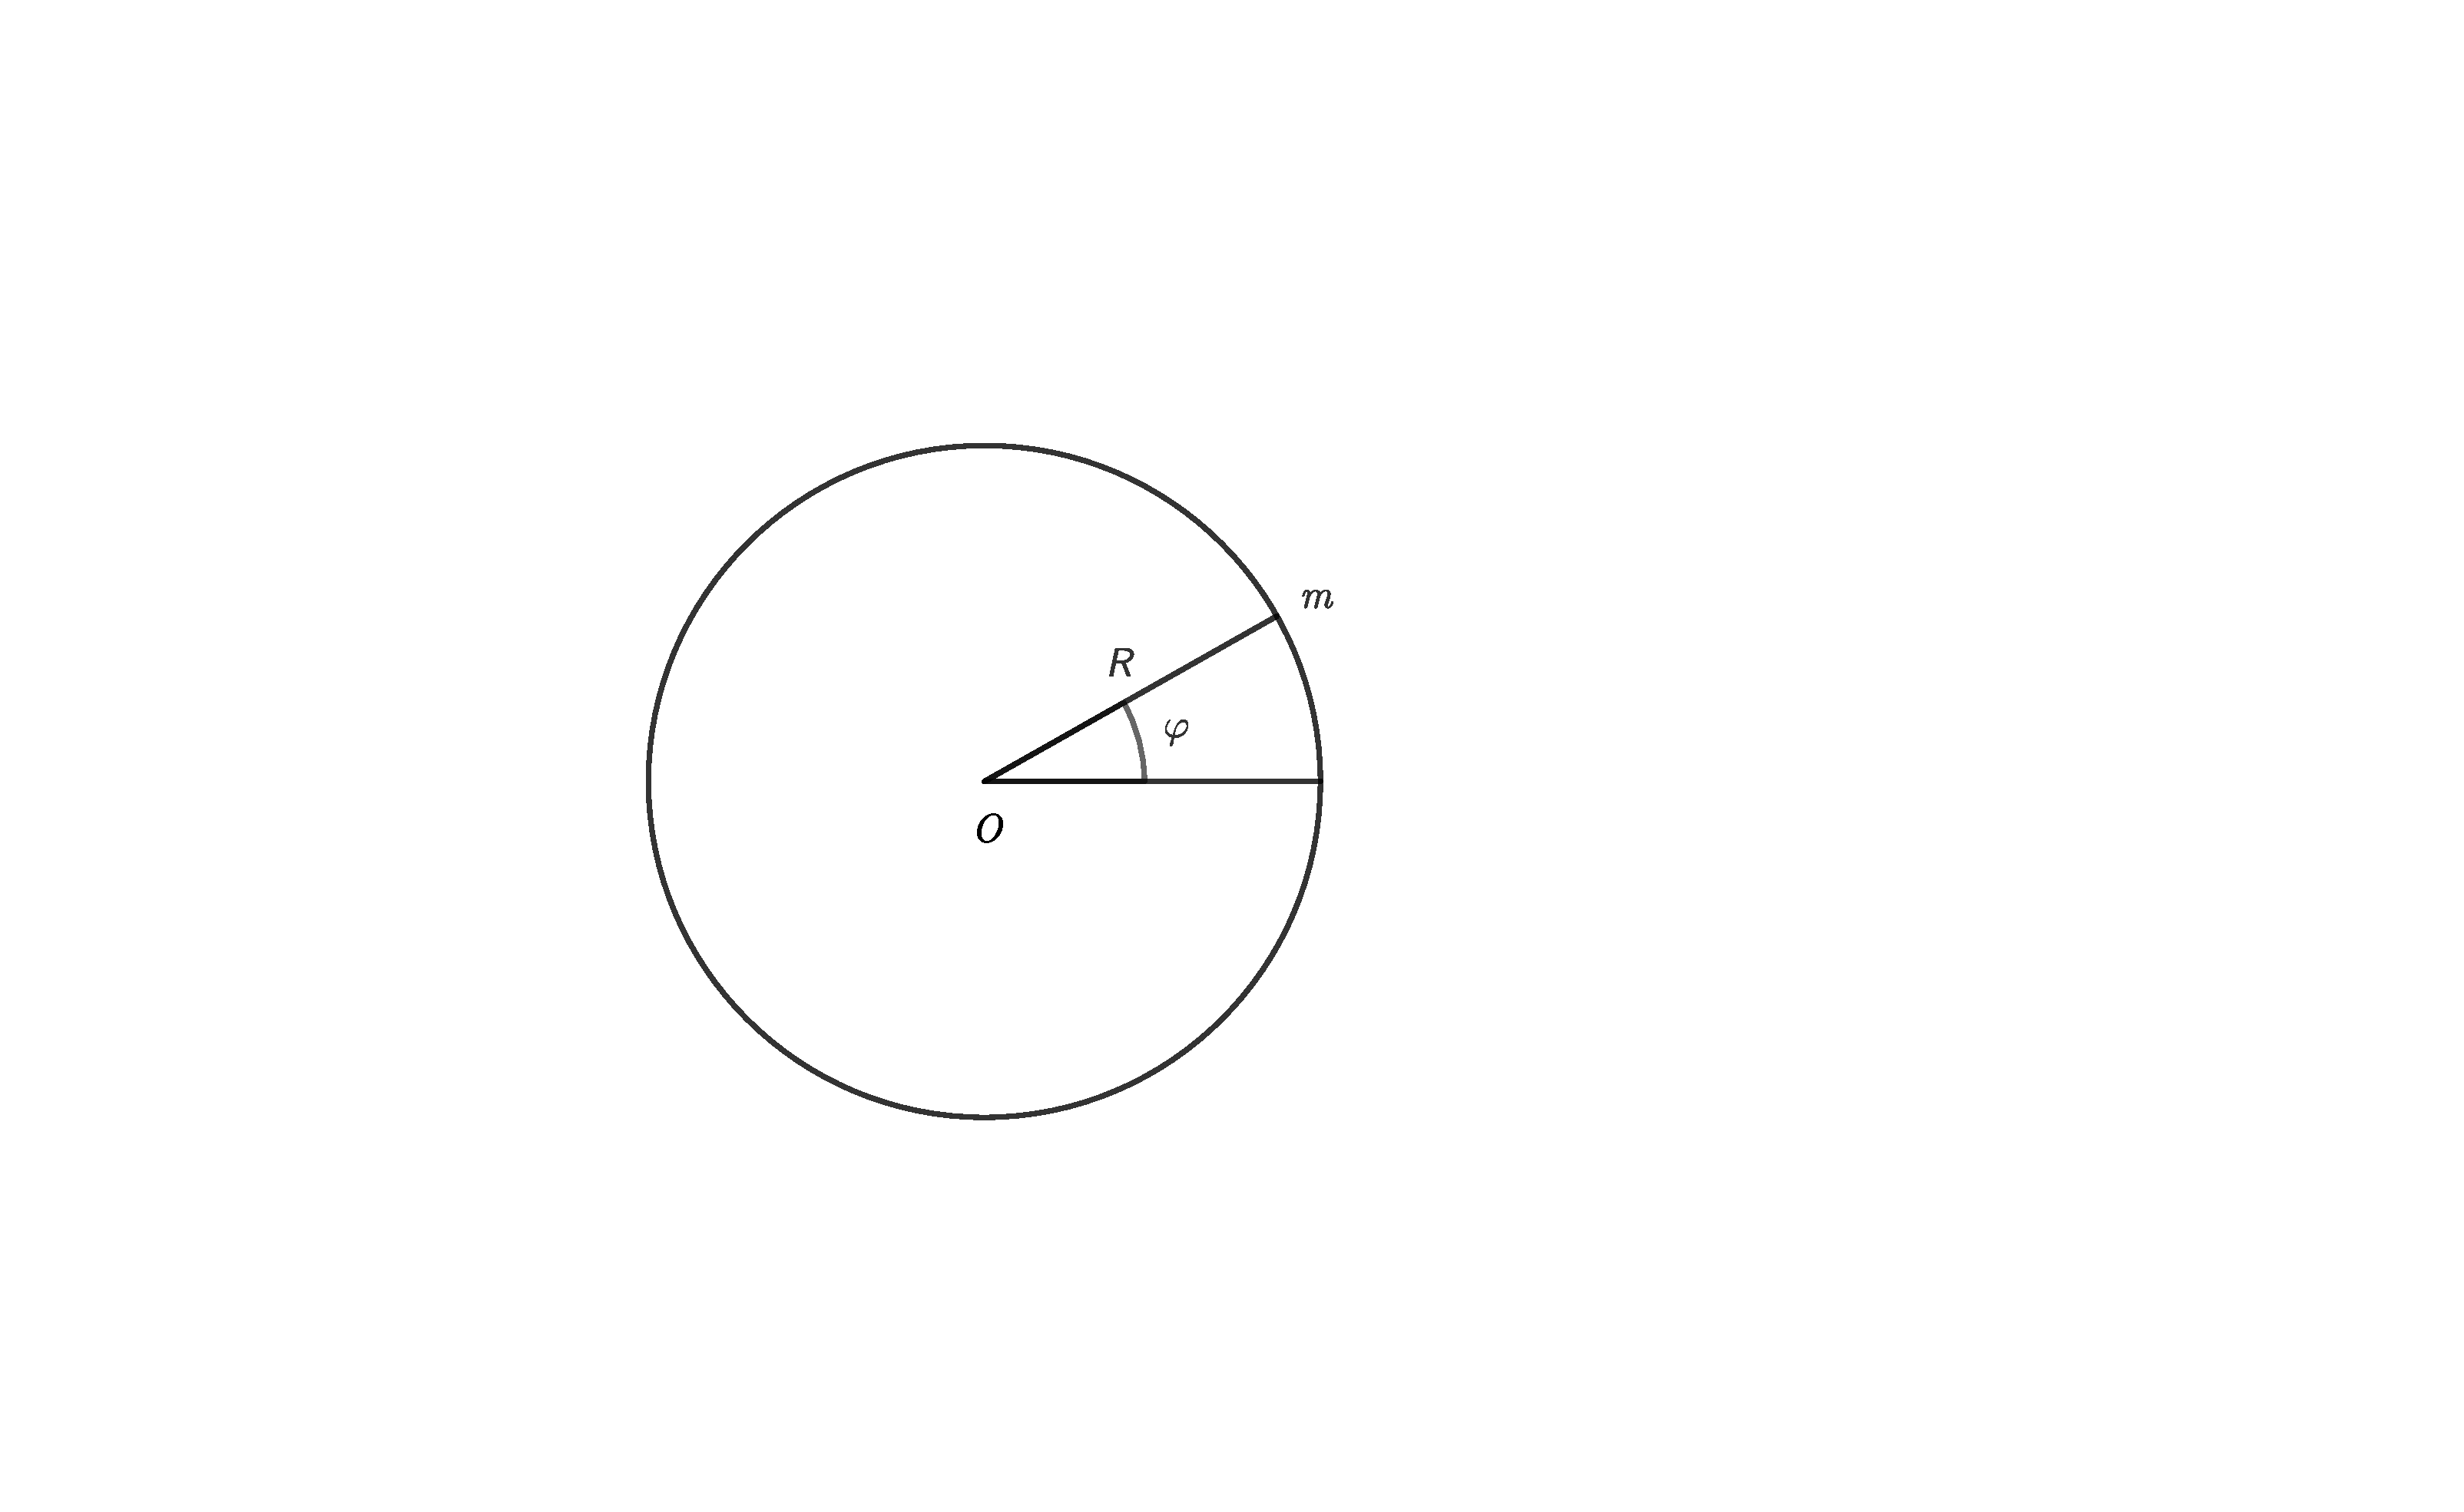
\includegraphics[width=2.5cm,clip]{QM file/figure/2-12}
	\caption{2-6题图}
	\label{fig.2-12}
\end{wrapfigure}

\exercise\label{ex2.6} 质量为$m$的粒子只能沿圆环(半径$R$)运动(如图\ref{fig.2-12}),能量算符为$\hat{H}=-\dfrac{\hbar^{2}}{2mR^{2}}\dfrac{d^{2}}{d\varphi^{2}}$,$\varphi$为旋转角.求能级($E_{n}$)及归一化函数$\varPsi_{n}(\varphi)$.讨论各能级的简并度.

本题是一种“平面转子”模型.平面转子的能量算符为
\begin{empheq}{equation*}
	\hat{H}=\frac{\hat{L}_{z}^{2}}{2I}=-\frac{\hbar^{2}}{2I}\frac{d^{2}}{d\varphi^{2}}
\end{empheq}
(在$x-y$面上旋转,转轴为$z$轴)其中$I$为转动惯量.

\exercise 对于一维运动,分布宽度$\Delta x$定义为
\begin{empheq}{equation*}
	\Delta x=(\bar{x^{2}}-\bar{x}^{2})^{\frac{1}{2}}
\end{empheq}
试对$\S$\ref{sec:02.04}中(1.)所讲的以及2-5题所求得的无限深势阱中的束缚态$\varPsi_{n}$,计算分布宽度$\Delta x$,并和经典力学的结论比较.
	
\begin{wrapfigure}[3]{r}{10em}
	\centering
	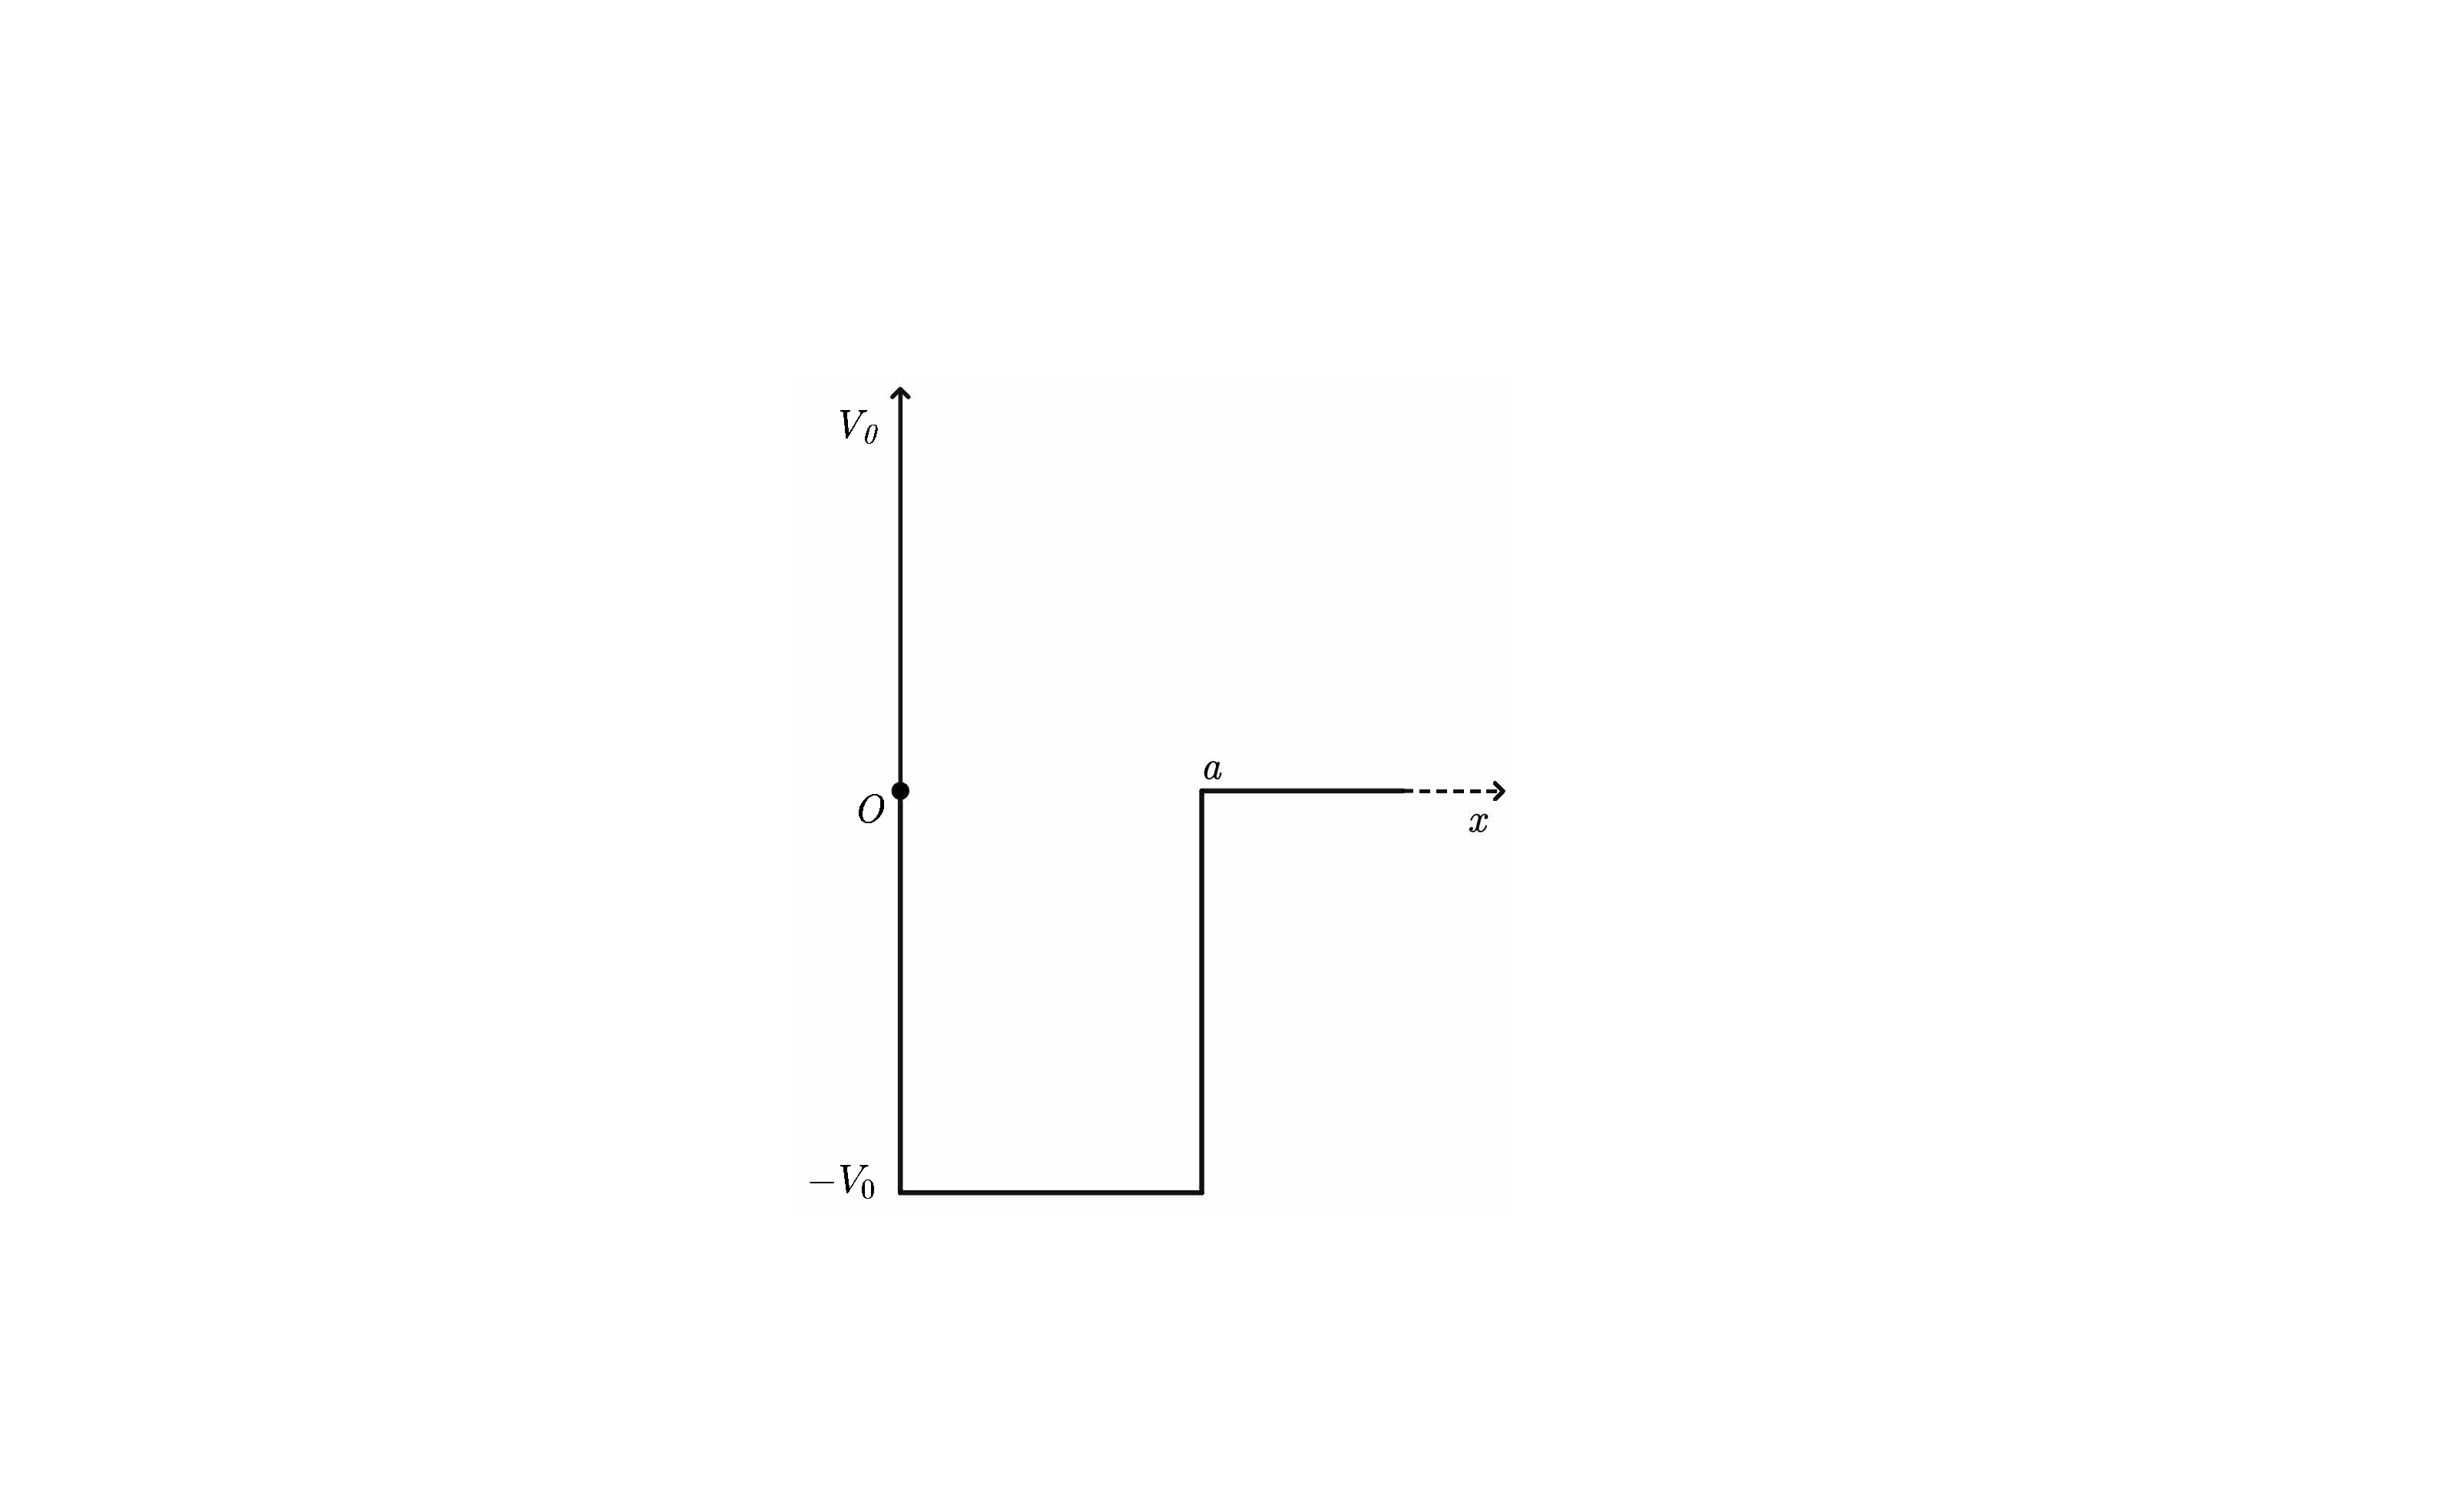
\includegraphics[width=3cm,clip]{QM file/figure/2-13}
	\caption{2-9题图}
	\label{fig.2-13}
\end{wrapfigure}
	
\exercise 对于$\delta$势阱造成的束缚态,计算$\bar{T},\bar{V},\Delta x,\Delta \boldsymbol{p}$.(定义见2-14题.)
	
\exercise 粒子在下列势阱中运动,
\setlength{\mathindent}{4em}
\begin{empheq}{equation*}
	V(x)=
	\begin{dcases}\notag
		\infty,	& x\geqslant 0	\\
		-V_{0}, & 0<x<a	\\
		0,		& x\leqslant a
	\end{dcases}
\end{empheq}\eqnormal
试证明仅当阱深、阱宽满足条件:
\setlength{\mathindent}{6em}
\begin{empheq}{equation*}
	V_{0}a^{2}>\frac{\hbar^{2}\pi^{2}}{8m}
\end{empheq}\eqnormal
时,才能存在束缚态($E<0$).并求能级方程.
	\pskip
\exercise 对于$\S$\ref{sec:02.04}中(2.)所讲有限深平底势阱,求

	(a)阱口刚好出现一个束缚态能级($E\approx0$)的条件.
	
	(b)束缚态能级总数,并和无限深势阱作比较.
	\pskip
\exercise 对于有限深平底势阱的第$n$个束缚态$\varPsi_{n}$,$E_{n}$,设$V_{0}\leqslant E_{n}+V_{0}$,计算

(a)粒子在阱外出现概率.

(b)$V(x)$和$V^{2}(x)$的平均值,并与$E_{n}$比较.
	\pskip
\exercise 对于谐振子的基态($\varPsi_{0}$)与第一激发态($\varPsi_{1}$),计算

(a)分布宽度$\Delta x$(定义见2-7题).

(b)粒子出现在经典禁区的概率.
	\pskip
\exercise 对于谐振子的能量本征态,证明下列公式
\begin{empheq}{equation*}
x\varPsi_{n}=\frac{x_{0}}{2}(\sqrt{n}\varPsi_{n-1}+\sqrt{n+1}\varPsi_{n+1})
\end{empheq}
\begin{empheq}{equation*}
	\frac{d}{dx}\varPsi_{n}=\frac{1}{\sqrt{2}x_{0}}(\sqrt{n}\varPsi_{n-1}-\sqrt{n+1}\varPsi_{n+1})
\end{empheq}

\exercise 利用上题中公式,求$\varPsi_{n}$的$\bar{T},\bar{V},\Delta x,\Delta \boldsymbol{p}$.$\Delta \boldsymbol{p}$定义为
\begin{empheq}{equation*}
	\Delta \boldsymbol{p}=(\bar{p_{x}^{2}}-\bar{p}_{x}^{2})^{\frac{1}{2}}
\end{empheq}

\exercise 二维各向同性谐振子,$\hat{H}=-\dfrac{\hbar^{2}}{2m}\bigg(\dfrac{\partial^{2}}{\partial x^{2}}+\dfrac{\partial^{2}}{\partial y^{2}}\bigg)+\dfrac{k}{2}(x^{2}+y^{2})$,试用分离变量法求能级和定态波函数,并求各能级的简并度.
	\pskip
\exercise 三维各向同性谐振子,$\hat{H}=-\dfrac{\hbar^{2}}{2m}\nabla^{2}+\dfrac{k}{2}(x^{2}+y^{2}+z^{2})$,试用分离变量法求能级和定态波函数,并讨论各能级的简并度.
	\pskip
\exercise 粒子在下列“切割谐振子势阱”中运动,
\begin{empheq}{equation*}
	V(x)=
	\begin{dcases}\notag
		\infty,				& x\geqslant 0	\\
		\frac{kx^{2}}{2},	& x>0
	\end{dcases}
\end{empheq}

求能级和定态波函数.

[提示:利用谐振子的结果.]

	\pskip
\exercise 二维耦合谐振子的能量算符为
\setlength{\mathindent}{5em}
\begin{empheq}{equation*}
	\hat{H}=\hat{T}+V=-\frac{\hbar^{2}}{2m}\bigg(\frac{\partial^{2}}{\partial x^{2}}+\frac{1}{2}m\omega^{2}(x^{2}+y^{2}\bigg)+\lambda xy
\end{empheq}\eqnormal

其中$|\lambda|<m\omega^{2}$.求能级.

[提示:作坐标变换$X=\dfrac{1}{\sqrt{2}}(x+y)$,$Y=\dfrac{1}{\sqrt{2}}(x-y)$容易证明:$\dfrac{\partial^{2}}{\partial x^{2}}+\dfrac{\partial^{2}}{\partial y^{2}}=\dfrac{\partial^{2}}{\partial X^{2}}+\dfrac{\partial^{2}}{\partial Y^{2}}$]

\newpage

\begin{wrapfigure}[9]{r}{10em}
	\centering
	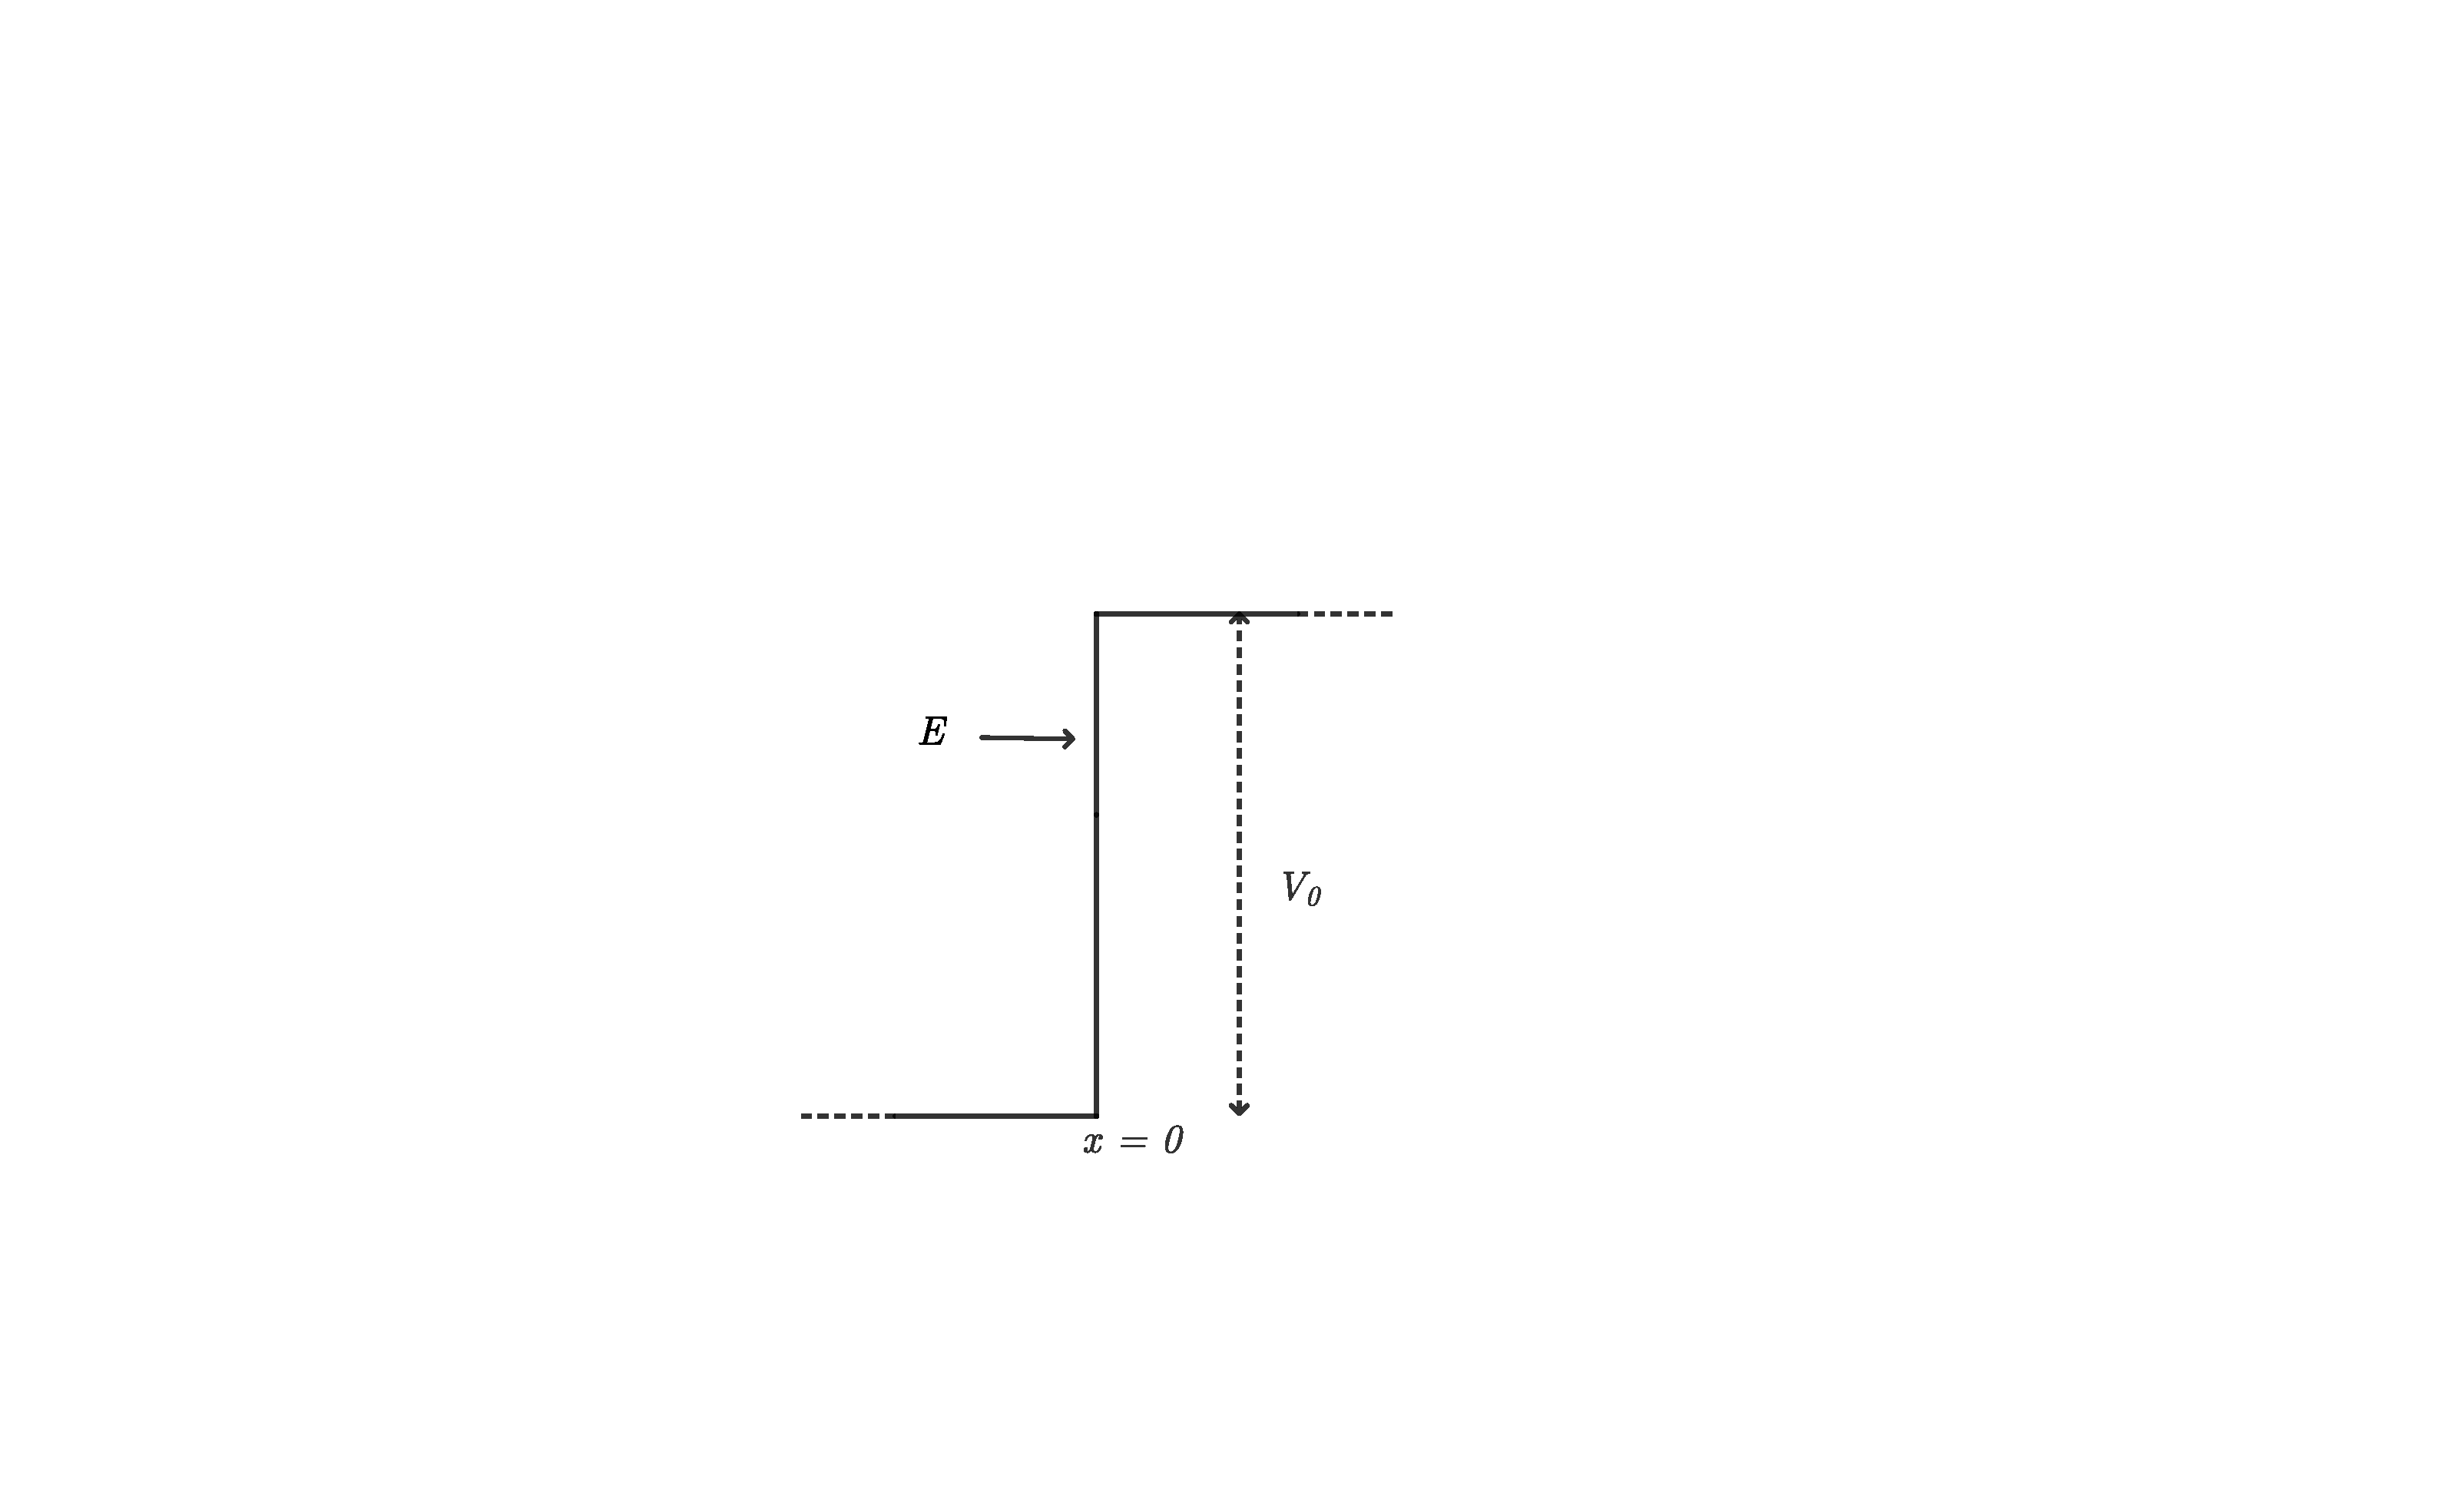
\includegraphics[width=3cm,clip]{QM file/figure/2-14}
	\caption{2-19题图}
	\label{fig.2-14}
\end{wrapfigure}
\exercise 粒子以动能$E=\dfrac{\hbar^{2}k^{2}}{2m}$从左方入射,遇势场(图\ref{fig.2-14})
\begin{empheq}{equation*}
	V(x)=
	\begin{dcases}\notag
		0,		& x<0	\\
		V_{0},	& x>0
	\end{dcases}
\end{empheq}

求反射系数和透射系数.($E>V_{0}$及$E<V_{0}$分别讨论.)
	\pskip
	\pskip
\exercise 粒子以动能$E=\dfrac{\hbar^{2}k^{2}}{2m}$从左方入射,遇$\delta$势垒$V(x)=\gamma\delta(x)$,$\gamma>0$,求透射系数.
\end{exercises}